\documentclass[se,manuscript]{copernicus}
\begin{document}

\setcounter{figure}{0}
\renewcommand{\thefigure}{S\arabic{figure}}
\setcounter{table}{0}
\renewcommand{\thetable}{S\arabic{table}}
\makeatletter
\let\ftype@table\ftype@figure
\makeatother

\title{Supporting information: Seismic amplitude response to internal heterogeneity of mass-transport deposits}

\Author[1]{Jonathan}{Ford}
\Author[1]{Angelo}{Camerlenghi}
\Author[2]{Francesca}{Zolezzi}
\Author[2]{Marilena}{Calarco}

\affil[1]{National Institute of Oceanography and Applied Geophysics -- OGS, Trieste, Italy}
\affil[2]{RINA Consulting, Genova, Italy}

\correspondence{J. Ford (jford@ogs.it)}

\runningtitle{Supporting Information}
\runningauthor{Ford et al.}

\received{}
\pubdiscuss{} %% only important for two-stage journals
\revised{}
\accepted{}
\published{}

\maketitle

\section*{Contents of this file}

\begin{enumerate}
    \item Black Sea case study area additional data:
    \begin{enumerate}
        \item Multi-sensor core logger (MSCL) data for four sediment cores (Fig.~\ref{fig:mscl})
        \item Cone penetration test (CPT) data for site GH-T-PCPT7 (Fig.~\ref{fig:cpt})
        \item Stacking velocity function from close to the alongslope sub-bottom profile (Fig.~\ref{fig:stacking-velocities})
    \end{enumerate}
    \item Synthetic modelling trace envelope results for all realisations:
    \begin{enumerate}
        \item Single-source experiment (Fig.~\ref{fig:single-source-1})
        \item Multi-source experiment (Fig.~\ref{fig:multi-source-3021})
    \end{enumerate}
    \item Model details and summary results for variations on the single-source synthetic experiment:
    \begin{enumerate}
        \item `Low-reflectivity' experiment (Table~\ref{table:single-source-low-reflectivity-parameters} and Fig.~\ref{fig:single-source-low-reflectivity})
        \item `High-reflectivity' experiment (Table~\ref{table:single-source-high-reflectivity-parameters} and Fig.~\ref{fig:single-source-high-reflectivity})
        \item `Far source' experiment (Table~\ref{table:single-source-deep-parameters}, Figs.~\ref{fig:single-source-deep-model} and \ref{fig:single-source-deep-results})
        \item `Low Poisson's ratio' experiment (Table~\ref{table:single-source-low-p-parameters} and Fig.~\ref{fig:single-source-low-poisson})
        \item Cross-plot between the single-source synthetic experiment and experiments (a) to (d) 
        of RMS amplitudes within the heterogeneous zone (Fig.~\ref{fig:single-source-xplot})
    \end{enumerate}
    \item Compute requirements for the synthetic modelling experiments (Table~\ref{table:compute})
\end{enumerate}


\begin{figure*}
    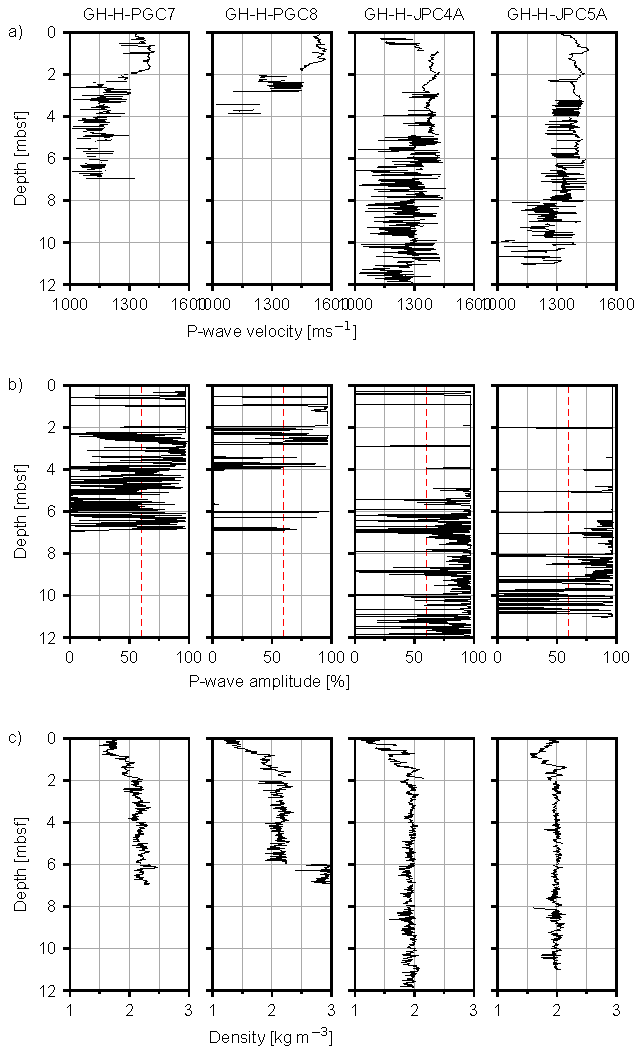
\includegraphics{figures/si_fig01_pg_1.pdf}
    \caption{Multi-sensor core logger (MSCL) results from cores GH-H-PGC7, GH-H-PGC8, GH-H-JPC4A and GH-H-JPB5A. a) P-wave velocity, b) P-wave amplitude (60\% cutoff marked), c) density, d) cross-plot of P-wave velocity and density logs, for depth intervals where the P-wave amplitude exceeds the 60\% cutoff. Parameter distributions are used to derive geologically plausible P-impedance contrasts for the two component sediment lithologies used in the multi-source synthetic experiment (Section 3.2) (cont.)}
    \label{fig:mscl}
\end{figure*}

\setcounter{figure}{0}

\begin{figure*}
    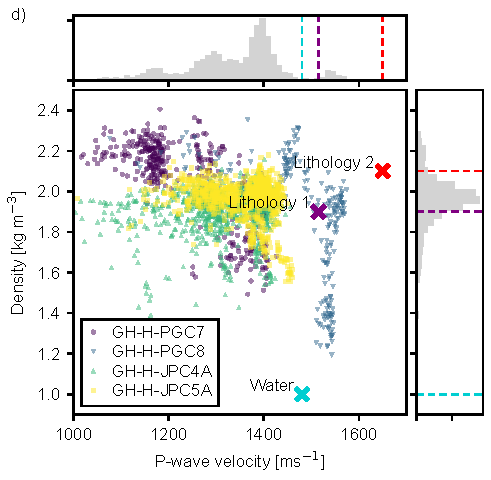
\includegraphics{figures/si_fig01_pg_2.pdf}
    \caption{}
\end{figure*}

\clearpage

\begin{figure*}
    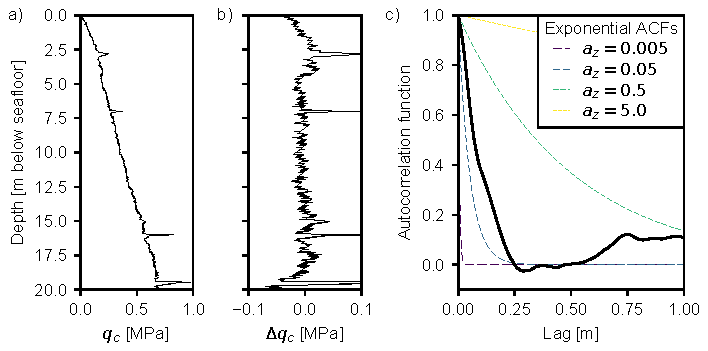
\includegraphics{figures/si_fig02.pdf}
    \caption{Cone-penetration test (CPT) results for site GH-T-PCPT7. a) Cone-tip resistance ($q_c$) log, b) De-trended cone-tip resistance log ($\Delta q_c$), de-trended with a best fit linear trend, c) Autocorrelation function (ACF) of the cone-tip resistance log.}
    \label{fig:cpt}
\end{figure*}

\clearpage

\begin{figure*}
    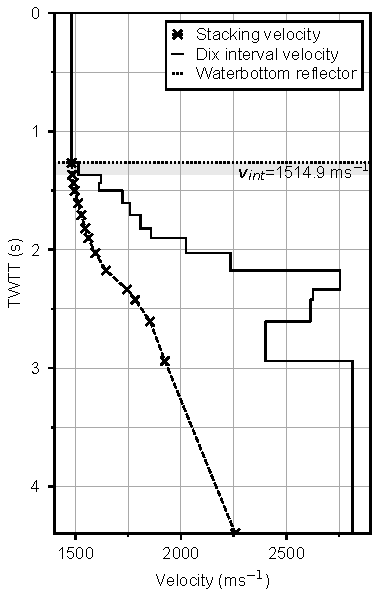
\includegraphics{figures/si_fig13.pdf}
    \caption{Picked NMO stacking velocities for a common mid-point gather from a multi-channel seismic reflection profile located close to the alongslope Black Sea sub-bottom profile (location in Fig.~1a).
    The water velocity is 1480 \unit{ms^{-1}}, and the average Dix-converted interval velocity ($v_{int}$) for 100 \unit{ms} beneath the seafloor (shaded grey) is marked.
    `TWTT' corresponds to two-way traveltime.}
    \label{fig:stacking-velocities}
\end{figure*} 

\clearpage

\begin{figure*}
    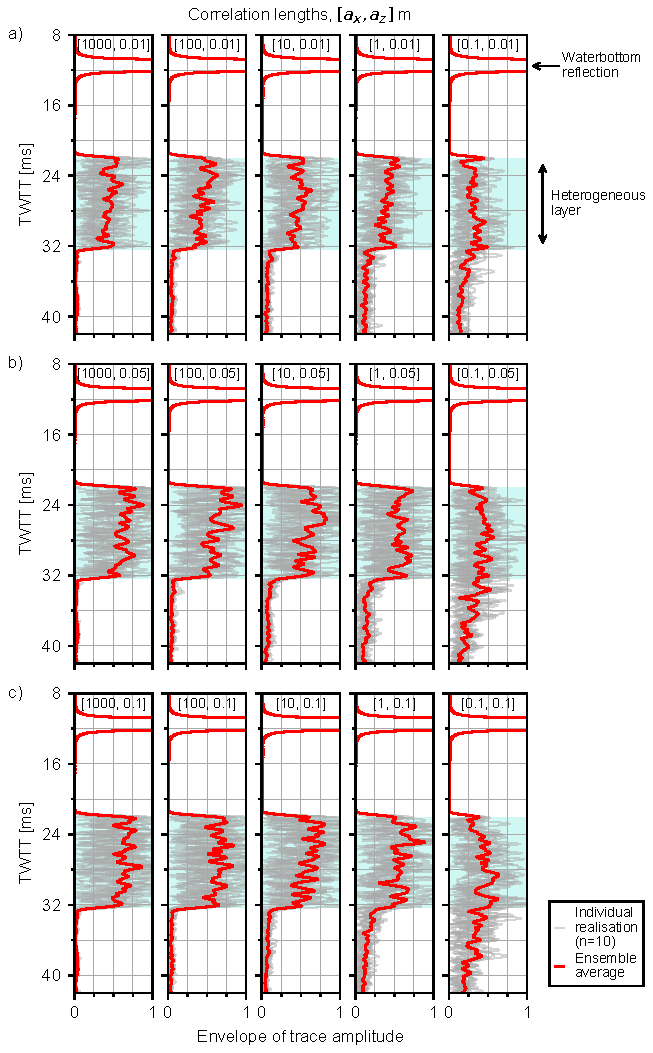
\includegraphics{figures/si_fig03_pg_1.pdf}
    \caption{Envelope of trace amplitude for individual realisations (grey) and the RMS envelope of the single-source synthetic experiment for each unique set of correlation lengths (red) for a range of vertical correlation lengths $a_z=\{0.01, 0.05, 0.1, 0.5, 1\}$ m (a-e) and lateral correlation lengths $a_x=\{1000, 100, 10, 1, 0.1\}$ \unit{m} (left to right).
    The two-way traveltime (TWTT) extent of the heterogeneous layer is shaded in blue. (cont.)}
    \label{fig:single-source-1}
\end{figure*}

\setcounter{figure}{3}

\begin{figure*}
    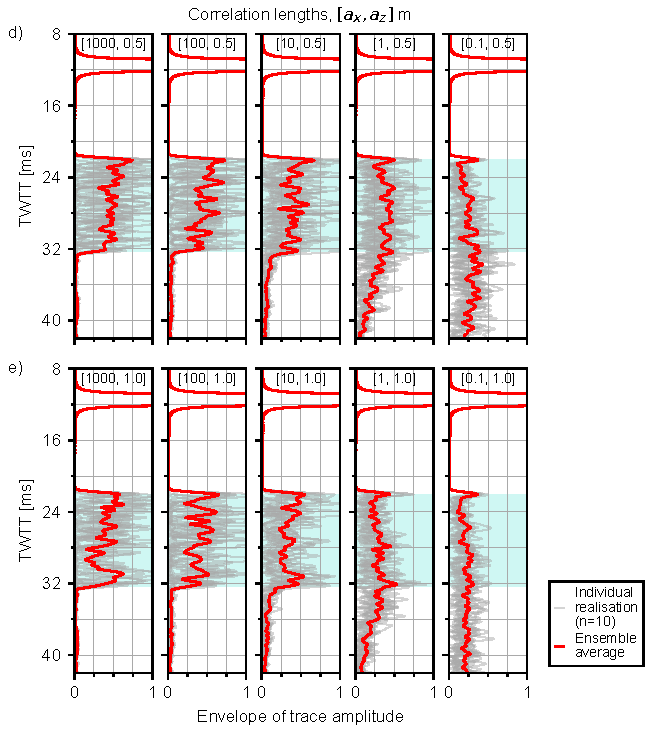
\includegraphics{figures/si_fig03_pg_2.pdf}
    \caption{}
    \label{fig:single-source-2}
\end{figure*}

\clearpage

\begin{figure*}
    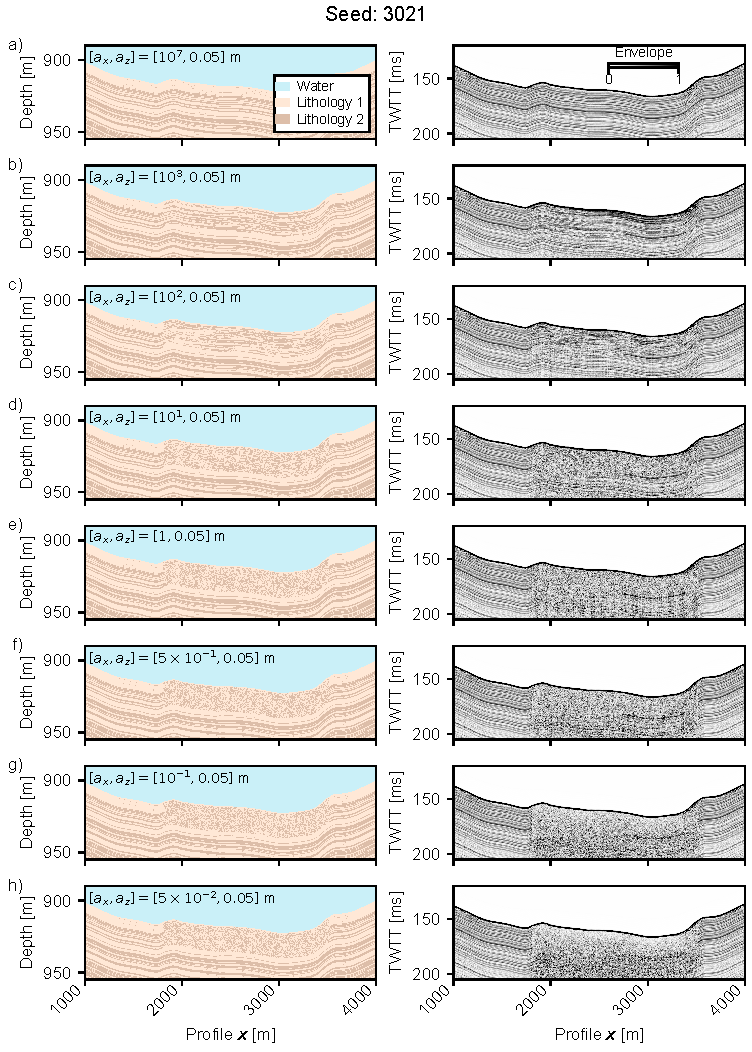
\includegraphics{figures/si_fig04.pdf}
    \caption{Realisations of the multi-source synthetic experiment models (left) and resulting synthetic sub-bottom profiles (right) for seed 3021, lateral scale lengths $a_x=\{1 \times 10^7 \text{(unfailed)}, 1000, 100, 10, 1, 0.5, 0.1, 0.05\}$ (a-h) and vertical scale length $a_z=0.05$ m.}
    \label{fig:multi-source-3021}
\end{figure*}

\begin{figure*}
    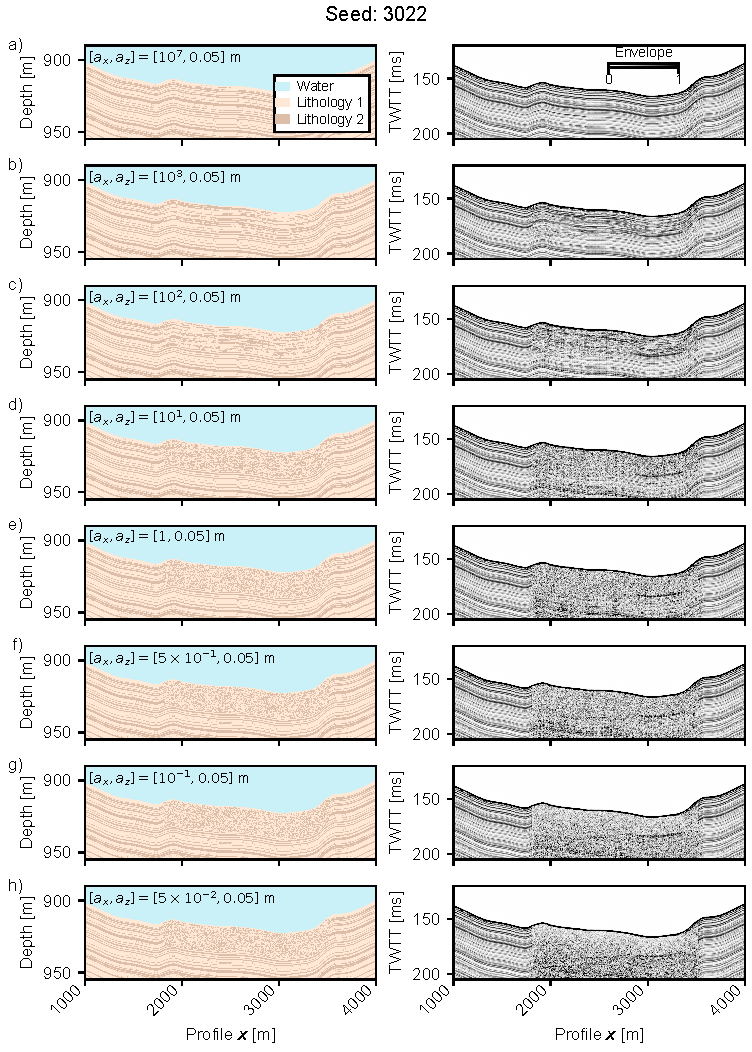
\includegraphics{figures/si_fig05.pdf}
    \caption{Realisations of the multi-source synthetic experiment models (left) and resulting synthetic sub-bottom profiles (right) for seed 3022, lateral scale lengths $a_x=\{1 \times 10^7 \text{(unfailed)}, 1000, 100, 10, 1, 0.5, 0.1, 0.05\}$ (a-h) and vertical scale length $a_z=0.05$ m.}
    \label{fig:multi-source-3022}
\end{figure*} 

\begin{figure*}
    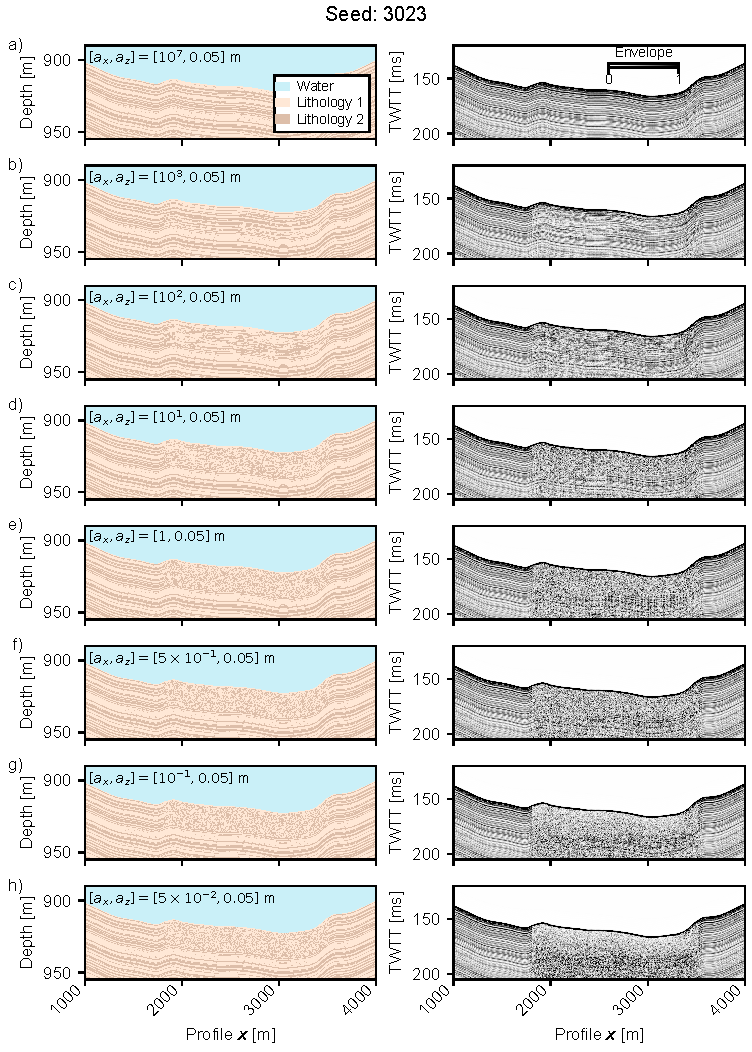
\includegraphics{figures/si_fig06.pdf}
    \caption{Realisations of the multi-source synthetic experiment models (left) and resulting synthetic sub-bottom profiles (right) for seed 3023, lateral scale lengths $a_x=\{1 \times 10^7 \text{(unfailed)}, 1000, 100, 10, 1, 0.5, 0.1, 0.05\}$ (a-h) and vertical scale length $a_z=0.05$ m.}
    \label{fig:multi-source-3023}
\end{figure*}

\begin{figure*}
    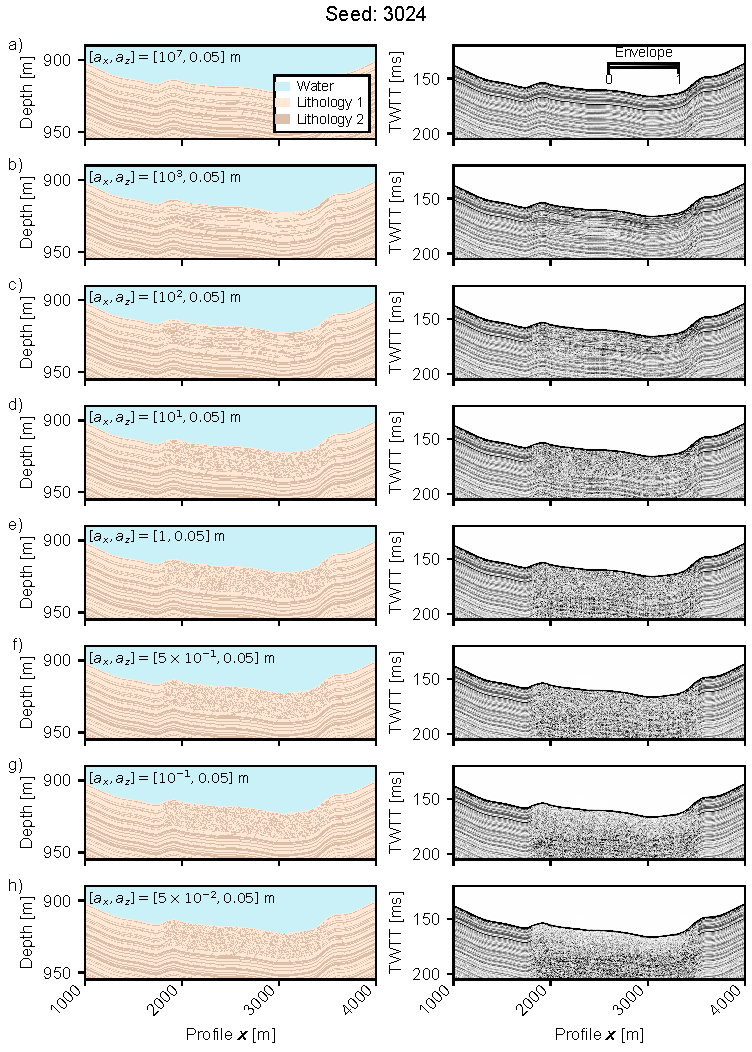
\includegraphics{figures/si_fig07.pdf}
    \caption{Realisations of the multi-source synthetic experiment models (left) and resulting synthetic sub-bottom profiles (right) for seed 3024, lateral scale lengths $a_x=\{1 \times 10^7 \text{(unfailed)}, 1000, 100, 10, 1, 0.5, 0.1, 0.05\}$ (a-h) and vertical scale length $a_z=0.05$ m.}
    \label{fig:multi-source-3024}
\end{figure*}

\begin{figure*}
    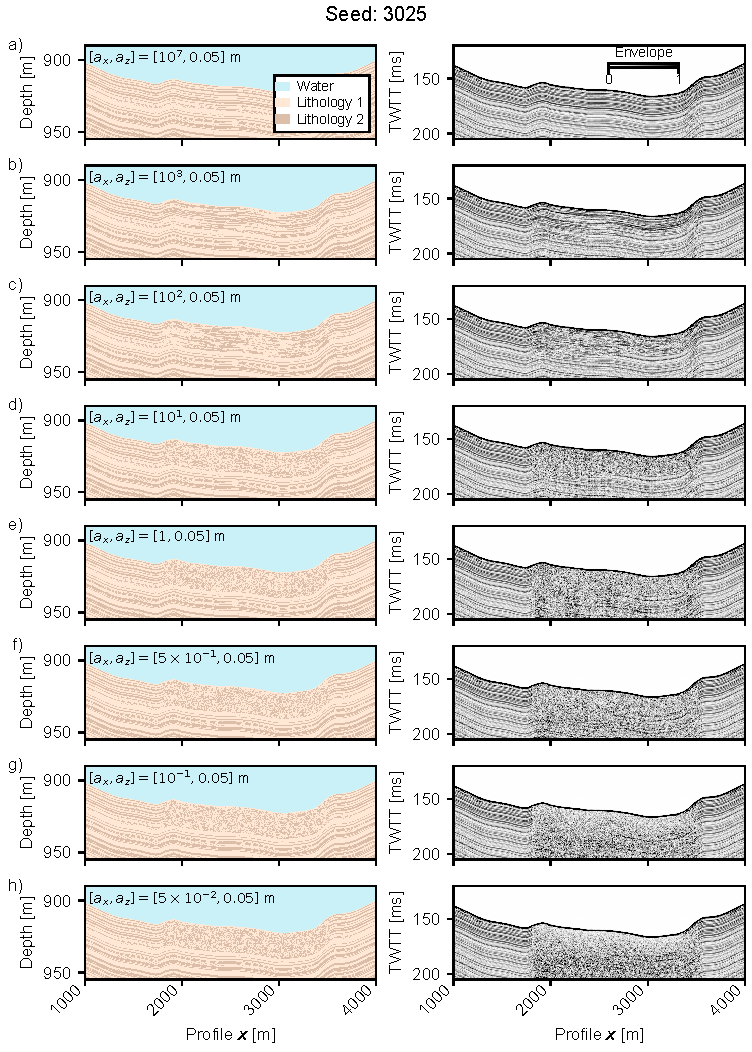
\includegraphics{figures/si_fig08.pdf}
    \caption{Realisations of the multi-source synthetic experiment models (left) and resulting synthetic sub-bottom profiles (right) for seed 3025, lateral scale lengths $a_x=\{1 \times 10^7 \text{(unfailed)}, 1000, 100, 10, 1, 0.5, 0.1, 0.05\}$ (a-h) and vertical scale length $a_z=0.05$ m.}
    \label{fig:multi-source-3025}
\end{figure*}

\clearpage
% Low reflectivity

\begin{table}
    \caption{Modelling parameters for the `low reflectivity' single-source synthetic experiment, including the elastic parameters for the water layer and the two sediment lithologies. The model geometry is identical to the single-source experiment (Fig. 3).}
    \label{table:single-source-low-reflectivity-parameters}
    \begin{tabular}{llll}
        \tophline
        \textbf{Component lithologies} & P-wave velocity & S-wave velocity & Density \\
        \middlehline
        Water & 1480 \unit{ms^{-1}} & --- & 1000 \unit{kg m^{-3}} \\
        Lithology 1 & 1515 \unit{ms^{-1}} & 379 \unit{ms^{-1}} & 1900 \unit{kg m^{-3}} \\
        Lithology 2 & 1550 \unit{ms^{-1}} & 388 \unit{ms^{-1}} & 1950 \unit{kg m^{-3}} \\
        \middlehline
        \textbf{Finite-difference modelling parameters} \\
        \middlehline
        Model dimensions & \multicolumn{3}{l}{40 $\times$ 40 \unit{m} (1601 $\times$ 1601 grid points)} \\
        Grid spacing & \multicolumn{3}{l}{0.025 $\times$ 0.025 \unit{m}} \\
        Timestep & \multicolumn{3}{l}{0.0089 \unit{ms}}\\
        Modelling time & \multicolumn{3}{l}{43.7 \unit{ms} (4908 timesteps)} \\
        Absorbing boundaries & \multicolumn{3}{l}{Sponge layers on all four grid edges} \\
        Source wavelet & \multicolumn{3}{l}{1.5 \unit{kHz} Ricker wavelet (zero-phase)} \\
        \bottomhline
    \end{tabular}
\end{table}

\begin{figure*}
    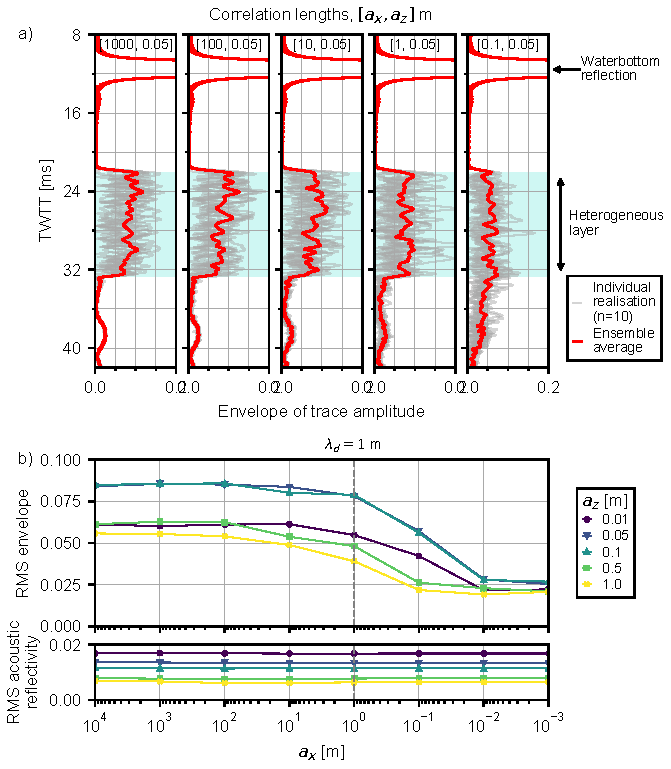
\includegraphics{figures/si_fig09.pdf}
    \caption{`Low reflectivity' single-source synthetic experiment results.
        a) Envelope of trace amplitude for $n=10$ multiple realisations (grey) and the RMS envelope of all realisations (red) for fixed vertical correlation length $a_z=0.05$ m and lateral correlation lengths $a_x=\{1000, 100, 10, 1, 0.1\}$ \unit{m} (from left to right).
        The two-way traveltime (TWTT) extent of the heterogeneous layer is shaded in blue.
        b) (Top) RMS envelope within the heterogeneous zone against lateral correlation length, $a_x$, grouped by vertical correlation length, $a_z$.
        (Bottom) RMS vertical incidence acoustic reflectivity within the heterogeneous zone.
        $\lambda_d$ shows the dominant wavelength of the seismic source in the sediment layers.
        Modelling parameters are given in Table~\ref{table:single-source-low-reflectivity-parameters}.}
    \label{fig:single-source-low-reflectivity}
\end{figure*}

\clearpage
% High reflectivity

\begin{table}
    \caption{Modelling parameters for the `high reflectivity' single-source synthetic experiment, including the elastic parameters for the water layer and the two sediment lithologies. The model geometry is identical to the single-source experiment (Fig. 3).}
    \label{table:single-source-high-reflectivity-parameters}
    \begin{tabular}{llll}
        \tophline
        \textbf{Component lithologies} & P-wave velocity & S-wave velocity & Density \\
        \middlehline
        Water & 1480 \unit{ms^{-1}} & --- & 1000 \unit{kg m^{-3}} \\
        Lithology 1 & 1515 \unit{ms^{-1}} & 379 \unit{ms^{-1}} & 1900 \unit{kg m^{-3}} \\
        Lithology 2 & 1800 \unit{ms^{-1}} & 450 \unit{ms^{-1}} & 2400 \unit{kg m^{-3}} \\
        \middlehline
        \textbf{Finite-difference modelling parameters} \\
        \middlehline
        Model dimensions & \multicolumn{3}{l}{40 $\times$ 40 \unit{m} (1601 $\times$ 1601 grid points)} \\
        Grid spacing & \multicolumn{3}{l}{0.025 $\times$ 0.025 \unit{m}} \\
        Timestep & \multicolumn{3}{l}{0.0080 \unit{ms}}\\
        Modelling time & \multicolumn{3}{l}{43.7 \unit{ms} (5470 timesteps)} \\
        Absorbing boundaries & \multicolumn{3}{l}{Sponge layers on all four grid edges} \\
        Source wavelet & \multicolumn{3}{l}{1.5 \unit{kHz} Ricker wavelet (zero-phase)} \\
        \bottomhline
    \end{tabular}
\end{table}

\begin{figure*}
    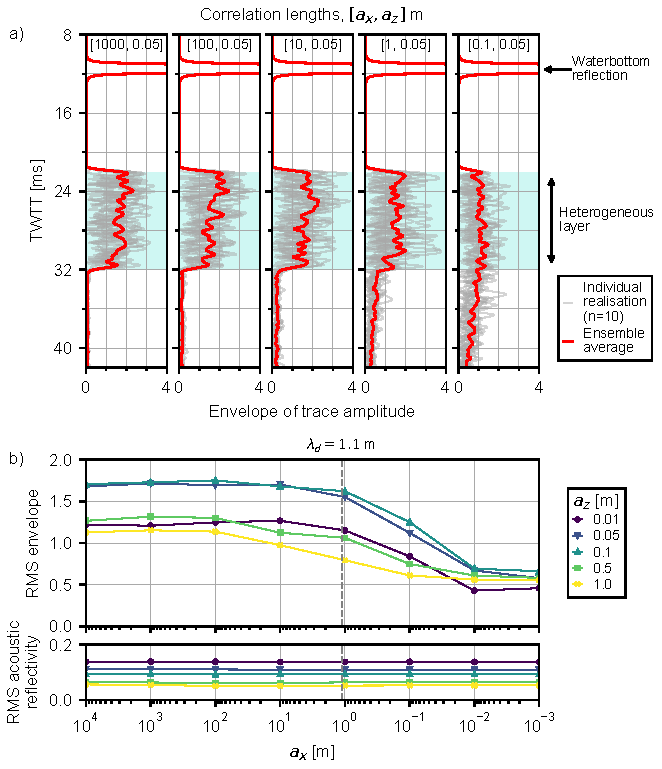
\includegraphics{figures/si_fig10.pdf}
    \caption{`High reflectivity' single-source synthetic experiment results.
        a) Envelope of trace amplitude for $n=10$ multiple realisations (grey) and the RMS envelope of all realisations (red) for fixed vertical correlation length $a_z=0.05$ m and lateral correlation lengths $a_x=\{1000, 100, 10, 1, 0.1\}$ \unit{m} (from left to right).
        The two-way traveltime (TWTT) extent of the heterogeneous layer is shaded in blue.
        b) (Top) RMS envelope within the heterogeneous zone against lateral correlation length, $a_x$, grouped by vertical correlation length, $a_z$.
        (Bottom) RMS vertical incidence acoustic reflectivity within the heterogeneous zone.
        $\lambda_d$ shows the dominant wavelength of the seismic source in the sediment layers.
        Modelling parameters are given in Table~\ref{table:single-source-high-reflectivity-parameters}.}
    \label{fig:single-source-high-reflectivity} 
\end{figure*}

\clearpage
% Deep

\begin{table}
    \caption{Modelling parameters for the `far source' single-source synthetic experiment, including the elastic parameters for the water layer and the two sediment lithologies.}
    \label{table:single-source-deep-parameters}
    \begin{tabular}{llll}
        \tophline
        \textbf{Component lithologies} & P-wave velocity & S-wave velocity & Density \\
        \middlehline
        Water & 1480 \unit{ms^{-1}} & --- & 1000 \unit{kg m^{-3}} \\
        Lithology 1 & 1515 \unit{ms^{-1}} & 379 \unit{ms^{-1}} & 1900 \unit{kg m^{-3}} \\
        Lithology 2 & 1650 \unit{ms^{-1}} & 413 \unit{ms^{-1}} & 2100 \unit{kg m^{-3}} \\
        \middlehline
        \textbf{Finite-difference modelling parameters} \\
        \middlehline
        Model dimensions & \multicolumn{3}{l}{80 $\times$ 80 \unit{m} (3201 $\times$ 3201 grid points)} \\
        Grid spacing & \multicolumn{3}{l}{0.025 $\times$ 0.025 \unit{m}} \\
        Timestep & \multicolumn{3}{l}{0.0089 \unit{ms}}\\
        Modelling time & \multicolumn{3}{l}{97.0 \unit{ms} (10915 timesteps)} \\
        Seismic source & \multicolumn{3}{l}{1.5 \unit{kHz} Ricker wavelet (zero-phase)} \\
        \bottomhline
    \end{tabular}
\end{table}

\begin{figure*}
    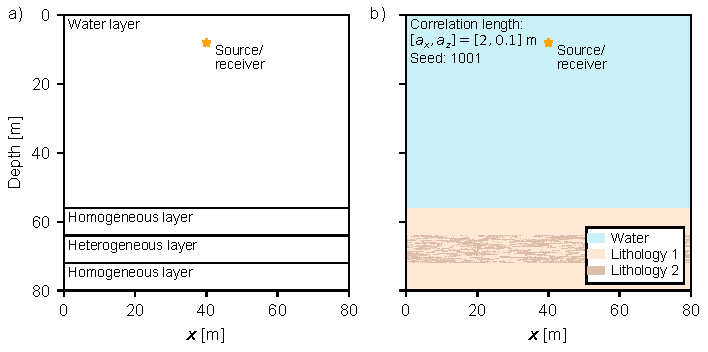
\includegraphics{figures/si_fig11.pdf}
    \caption{`Far source' single-source synthetic experiment.
        a) Model geometry. The coincident seismic source and receiver (yellow star) is located within the water layer, 56 \unit{m} from the top of the heterogeneous layer.
        b) A single realisation of the model showing the spatial distribution of Lithology 1 and Lithology 2 within the heterogeneous layer. Modelling parameters are listed in Table~\ref{table:single-source-deep-parameters}.}
    \label{fig:single-source-deep-model} 
\end{figure*}

\begin{figure*}
    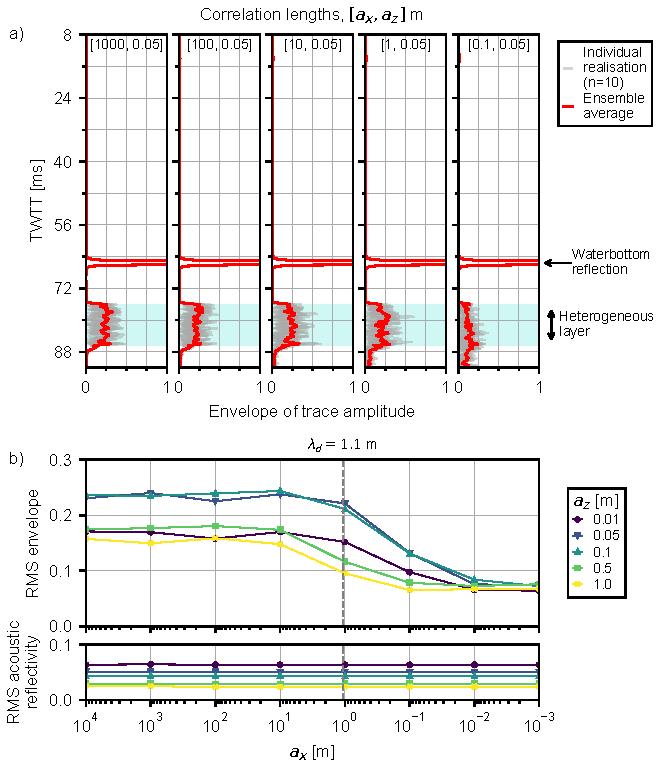
\includegraphics{figures/si_fig12.pdf}
    \caption{`Far source' single-source synthetic experiment results.
        a) Envelope of trace amplitude for $n=10$ multiple realisations (grey) and the RMS envelope of all realisations (red) for fixed vertical correlation length $a_z=0.05$ m and lateral correlation lengths $a_x=\{1000, 100, 10, 1, 0.1\}$ \unit{m} (from left to right).
        The two-way traveltime (TWTT) extent of the heterogeneous layer is shaded in blue.
        b) (Top) RMS envelope within the heterogeneous zone against lateral correlation length, $a_x$, grouped by vertical correlation length, $a_z$.
        (Bottom) RMS vertical incidence acoustic reflectivity within the heterogeneous zone.
        $\lambda_d$ shows the dominant wavelength of the seismic source in the sediment layers.
        Modelling parameters are given in Table~\ref{table:single-source-deep-parameters} and the model geometry is shown in Fig.~\ref{fig:single-source-deep-model}.}
    \label{fig:single-source-deep-results} 
\end{figure*}

\clearpage
% Low-p

\begin{table}
    \caption{Modelling parameters for the `low Poisson's ratio' single-source synthetic experiment, including the elastic parameters for the water layer and the two sediment lithologies. Poisson's ratio $\nu=0.33$ in the sediment layers, corresponding to $v_P/v_S=2$.}
    \label{table:single-source-low-p-parameters}
    \begin{tabular}{llll}
        \tophline
        \textbf{Component lithologies} & P-wave velocity & S-wave velocity & Density \\
        \middlehline
        Water & 1480 \unit{ms^{-1}} & --- & 1000 \unit{kg m^{-3}} \\
        Lithology 1 & 1515 \unit{ms^{-1}} & 758 \unit{ms^{-1}} & 1900 \unit{kg m^{-3}} \\
        Lithology 2 & 1650 \unit{ms^{-1}} & 825 \unit{ms^{-1}} & 2100 \unit{kg m^{-3}} \\
        \middlehline
        \textbf{Finite-difference modelling parameters} \\
        \middlehline
        Model dimensions & \multicolumn{3}{l}{40 $\times$ 40 \unit{m} (1601 $\times$ 1601 grid points)} \\
        Grid spacing & \multicolumn{3}{l}{0.025 $\times$ 0.025 \unit{m}} \\
        Timestep & \multicolumn{3}{l}{0.0081 \unit{ms}}\\
        Modelling time & \multicolumn{3}{l}{43.7 \unit{ms} (5401 timesteps)} \\
        Absorbing boundaries & \multicolumn{3}{l}{Sponge layers on all four grid edges} \\
        Source wavelet & \multicolumn{3}{l}{1.5 \unit{kHz} Ricker wavelet (zero-phase)} \\
        \bottomhline
    \end{tabular}
\end{table}

\begin{figure*}
    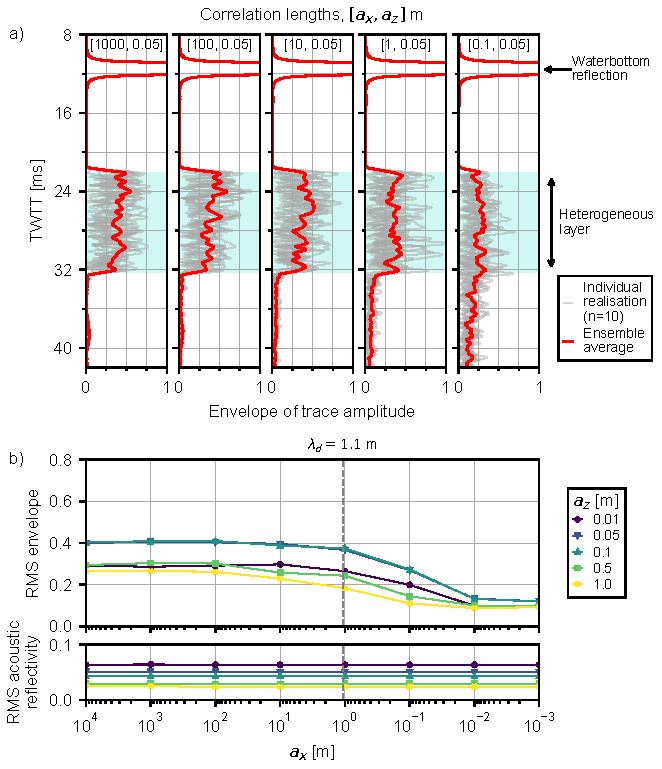
\includegraphics{figures/si_fig14.pdf}
    \caption{`Low Poisson's ratio' single-source synthetic experiment results, where $\nu=0.33$ in the sediment layers.
        a) Envelope of trace amplitude for $n=10$ multiple realisations (grey) and the RMS envelope of all realisations (red) for fixed vertical correlation length $a_z=0.05$ m and lateral correlation lengths $a_x=\{1000, 100, 10, 1, 0.1\}$ \unit{m} (from left to right).
        The two-way traveltime (TWTT) extent of the heterogeneous layer is shaded in blue.
        b) (Top) RMS envelope within the heterogeneous zone against lateral correlation length, $a_x$, grouped by vertical correlation length, $a_z$.
        (Bottom) RMS vertical incidence acoustic reflectivity within the heterogeneous zone.
        $\lambda_d$ shows the dominant wavelength of the seismic source in the sediment layers.
        Modelling parameters are given in Table~\ref{table:single-source-low-p-parameters}.}
    \label{fig:single-source-low-poisson} 
\end{figure*}

\begin{figure*}
    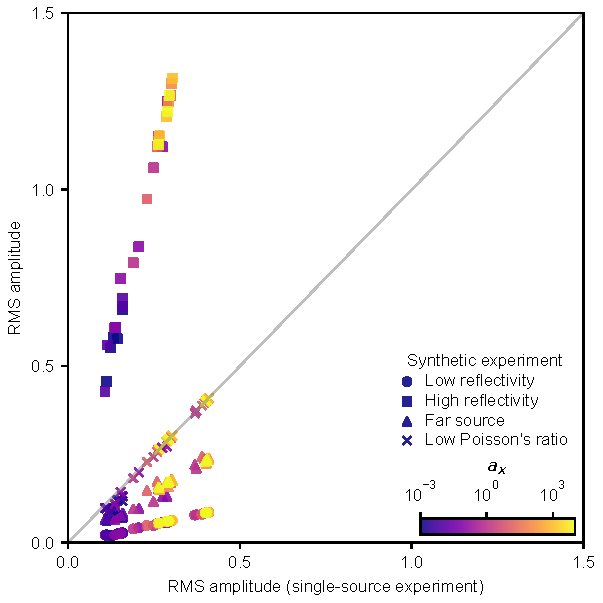
\includegraphics{figures/si_fig15.pdf}
    \caption{Cross-plot of the average RMS amplitudes within the heterogeneous zone, between the single-source experiment (Fig. 4) and the `low reflectivity' (Fig.~\ref{fig:single-source-low-reflectivity}), `high reflectivity' (Fig.~\ref{fig:single-source-high-reflectivity}), `far source' (Fig.~\ref{fig:single-source-deep-results}) and `low Poisson's ratio' (Fig.~\ref{fig:single-source-low-poisson}) synthetic experiments.}
    \label{fig:single-source-xplot} 
\end{figure*}

\clearpage
% Compute

\begin{table}
    \caption{Approximate computational runtimes for the single-source and multi-source experiments.
    Models were run on an HPC cluster with 48-core nodes (2 $\times$ 24-core Intel Xeon Platinum 8276-8276L) and 384 GB memory.
    Quoted CPU times are per logical CPU core.
    For the multi-source experiment, the runtime of each shot represents the average computation time for each sub-model, as the exact sub-model grid size depends on the source location within the global model (Section 3.2).
    Modelling runs for sub-models that are identical with changing $a_x$ (i.e., sub-models that do not overlap the MTD zone) are re-used, resulting in approximately 30\% reduction in compute time compared to modelling all sub-models.}
    \label{table:compute}
    \begin{tabular}{llll}
        \tophline
        Synthetic experiment & CPU time (single shot) & Number of shots & CPU time (total) \\
        \middlehline
        Single-source & \multirow{4}{*}{12 mins} & \multirow{4}{*}{400} & \multirow{4}{*}{80 hours} \\
        \hspace{\parindent} `Low reflectivity' & & & \\
        \hspace{\parindent} `High reflectivity' & & & \\
        \hspace{\parindent} `Low Poisson's ratio' & & & \\
        \middlehline
        `Far source' single-source & 1 hour & 400 & 420 hours \\
        \middlehline
        Multi-source & 10 mins & 37 224 modelled (+ 22 816 cached shots) & 6 200 hours \\
        \bottomhline
    \end{tabular}
\end{table}


\end{document}
